\pdfminorversion=4
\documentclass[]{article}
\usepackage[utf8]{inputenc}
\usepackage{amssymb,latexsym,amsmath}
\usepackage[a4paper,top=3cm,bottom=2cm,left=3cm,right=3cm,marginparwidth=1.75cm]{geometry}
\usepackage{graphicx}
\usepackage[colorlinks=true, allcolors=blue]{hyperref}
\begin{document}

\section{Name: Monisha C, Roll no: ME20B112}
\subsection{poisson's equation}~\cite{poisson's}
\begin{equation}
\nabla \cdot E = \frac{\rho_v}{\varepsilon} = \nabla^2 V
\end {equation}
\begin{flushleft}
$E$ = Electric \ field \\
$\rho$ = volume \ charge \ density \\
$\varepsilon$ = premittivity\\
$V$ = Electric \ Potential
\end{flushleft}

\paragraph{}
Note that Poisson’s Equation is a partial differential equation, and therefore can be solved using well-known techniques already established for such equations. In fact, Poisson’s Equation is an inhomogeneous differential equation, with the inhomogeneous part  −ρv/ϵ  representing the source of the field. In the presence of material structure, we identify the relevant boundary conditions at the interfaces between materials, and the task of finding  V(r)  is reduced to the purely mathematical task of solving the associated boundary value problem.


\begin{figure}[h]
\begin{center}
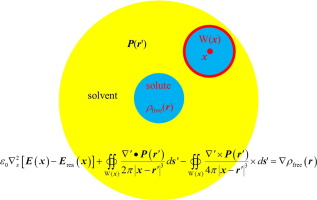
\includegraphics[width=200px]{ME20B112.jpg}
\caption{ME20B112}~\cite{me20b112}
\label{fig:poisson}
\end{center}
\end{figure}

\bibiliography{ME20B112.bib}
\bibiliographystyle{plain}


\end{document}

